\subsection{样本总体情况概览}
本次样本共收到 89 份有效回答,其中男女比例接近 1:1,
如图(\ref{pic:overall}\ref{sub@pic:gender})所示,
表明调查样本在性别分布上是相对均衡的,调查结果具有代表性。年龄段方面以大一学生为主,也有少量高年级学生,如图(\ref{pic:overall}\ref{sub@pic:age})所示。
\begin{figure}[H]
    \centering
    \subfigure[性别分布]{\label{pic:gender}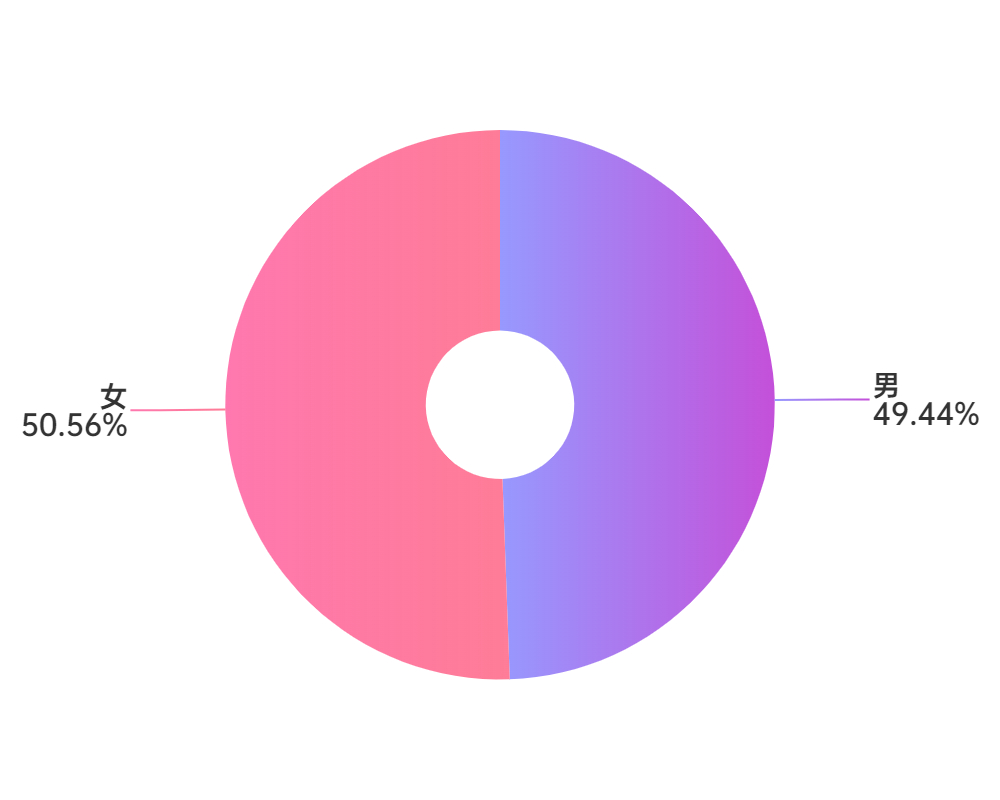
\includegraphics[width=0.4\textwidth]{./pic/性别分布.jpg}}
    \subfigure[年龄分布]{\label{pic:age}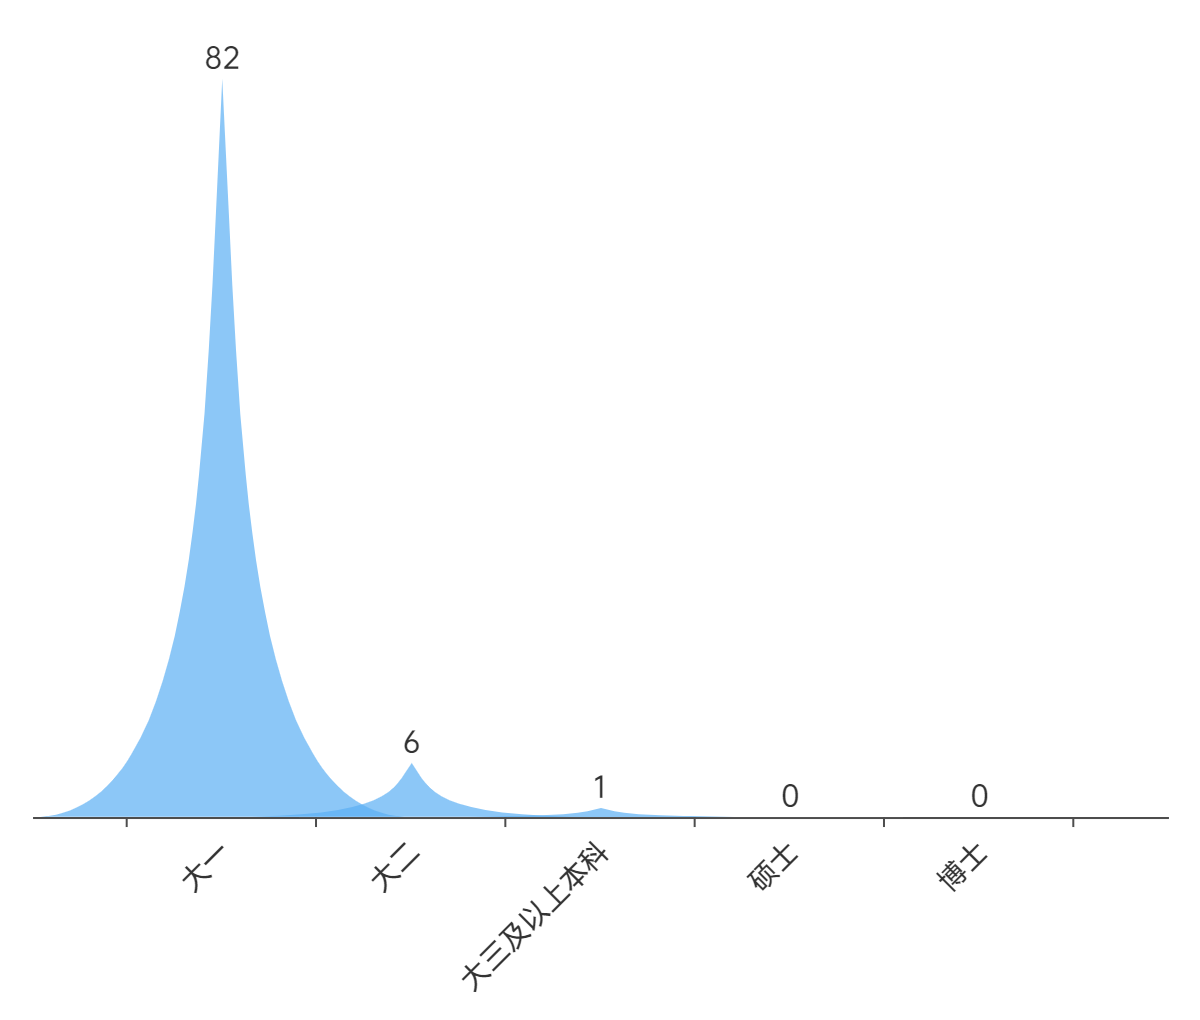
\includegraphics[width=0.4\textwidth]{./pic/年龄分布.png}}
    \caption{样本总体情况概览}
    \label{pic:overall}
\end{figure}

\subsection{对于化妆和医美的看法}
在对化妆和医美的态度上,近一半同学持中立态度,没有特别明显的喜憎表达,如图(\ref{pic:yimei})所示。
\begin{figure}[H]
    \centering
    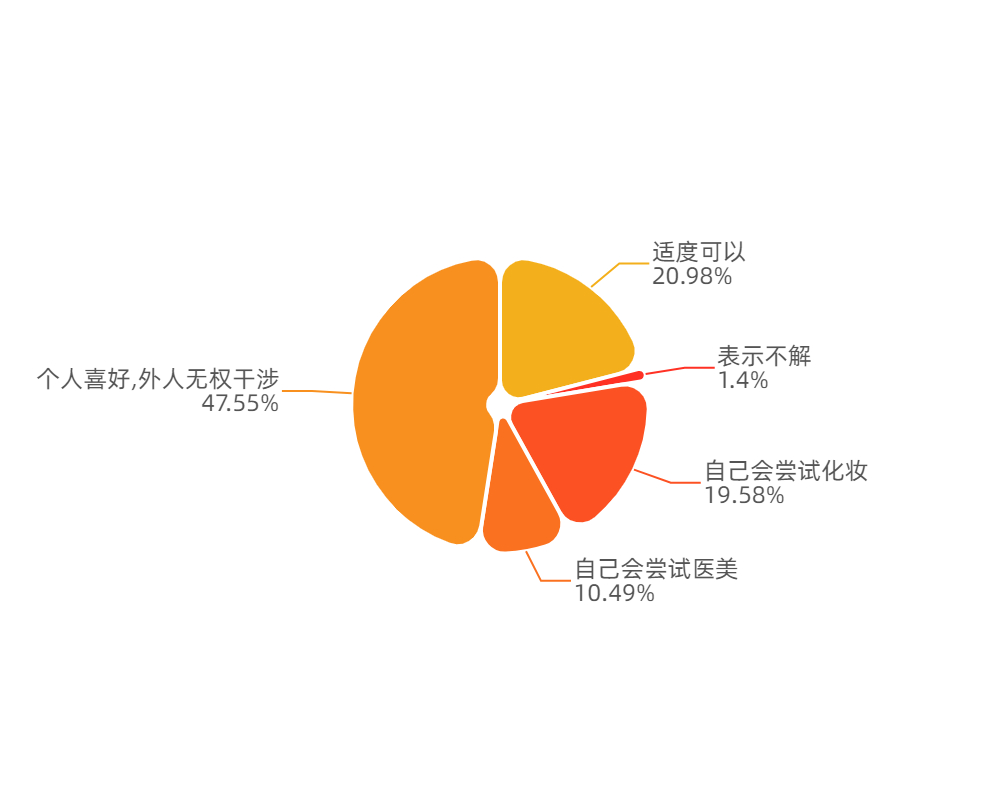
\includegraphics[width=0.4\textwidth]{./pic/对于化妆和医美的看法.jpg}
    \caption{对于化妆和医美的看法}
    \label{pic:yimei}
\end{figure}
\subsection{在整理容貌上花费的时间}
\begin{enumerate}[leftmargin=7em]
    \item 绝大部分同学不会花大量的时间

    根据数据分析,大多数人(93.26\%)每天在修饰自身容貌上花费的时间少于1.5小时,表明大部分人对个人形象的关注和维护是相对合理的。

    仅有4.49\%的人花费1.5小时到3小时,而超过3小时的人更是仅占2.25\%。

    \item 仅极少数同学会花较多时间,且这部分同学中,大部分为女生

    相较于男生群体,女生群体在整理修饰容貌上可能会需要更多的时间,也可能更倾向于在此方面投入较多时间。

\end{enumerate}
\begin{figure}[H]
    \centering
    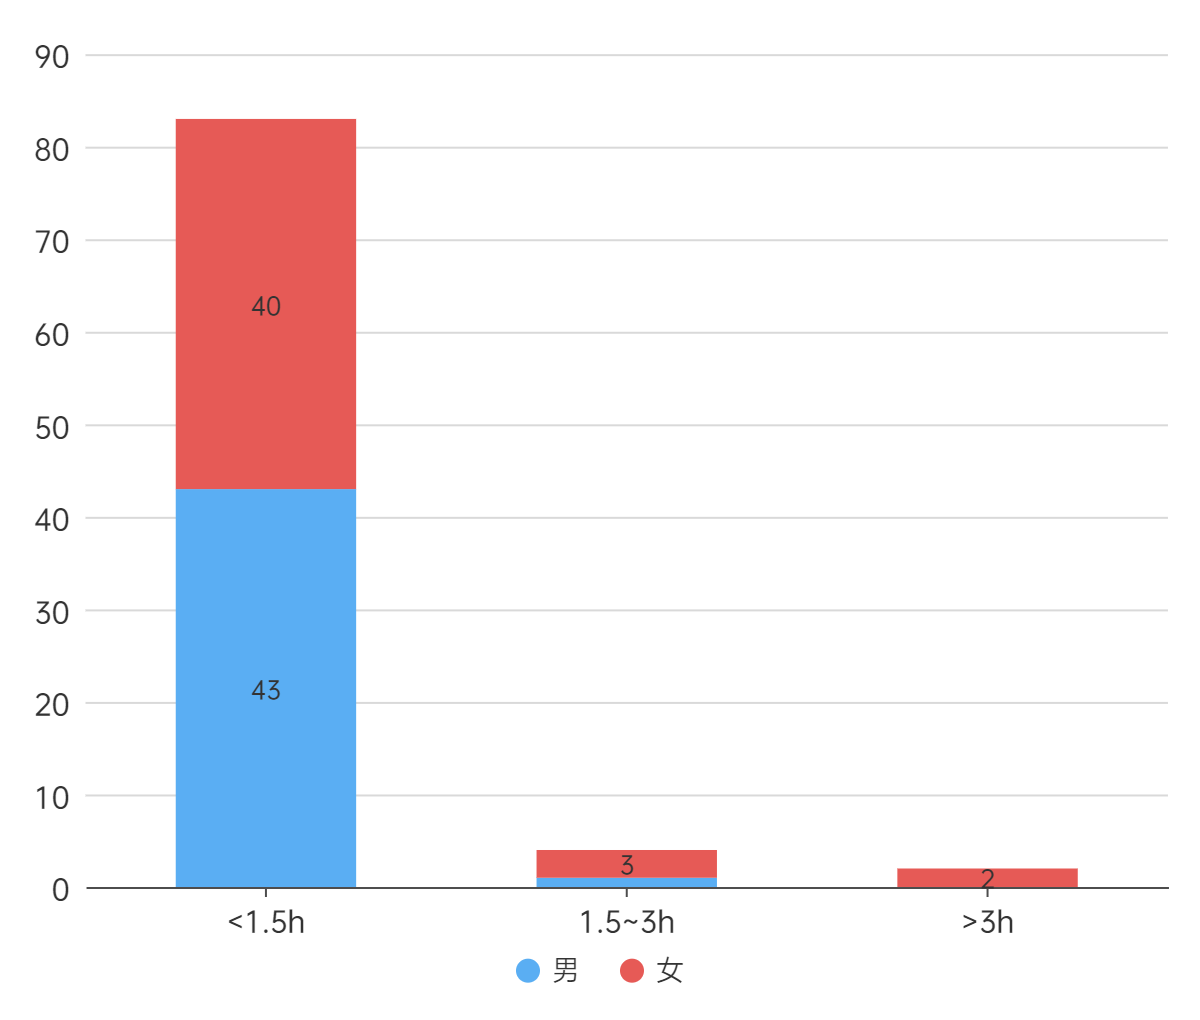
\includegraphics[width=.5\textwidth]{./pic/整理容貌所用的时间.png}
    \caption{整理容貌所用的时间}
    \label{pic:times}
\end{figure}
\subsection{对花时间整理容貌的看法}
\begin{enumerate}[leftmargin=7em]
    \item 大多数被试者(93.26\%)认为整理容貌可以改善精神面貌,
    表明新时期大学生群体大多能正视容貌的价值和作用,并认为外貌与精神状态之间存在一定的正相关关系。

    \item 少数(6.74\%)的被试者认为自己过于关注外貌,受到了负面影响。

    对于这类同学,我们进一步设问关于花费大量时间整理容貌的原因,得出以下结论:
    \begin{enumerate}
        \item 主要原因是\textbf{社会竞争压力增大},劳动力素质普遍得到提高,外在形象对于大学生群体的价值比重有所提升;
        \item 部分\textbf{男生}还认为是\textbf{恋爱}的导致的容貌需求;
        \item 部分\textbf{女生}认为更多的受到了\textbf{医美广告}、\textbf{化妆广告}及\textbf{网红的言论}和\textbf{视频}影响。
    \end{enumerate}
\end{enumerate}
\begin{figure}[H]
    \centering
    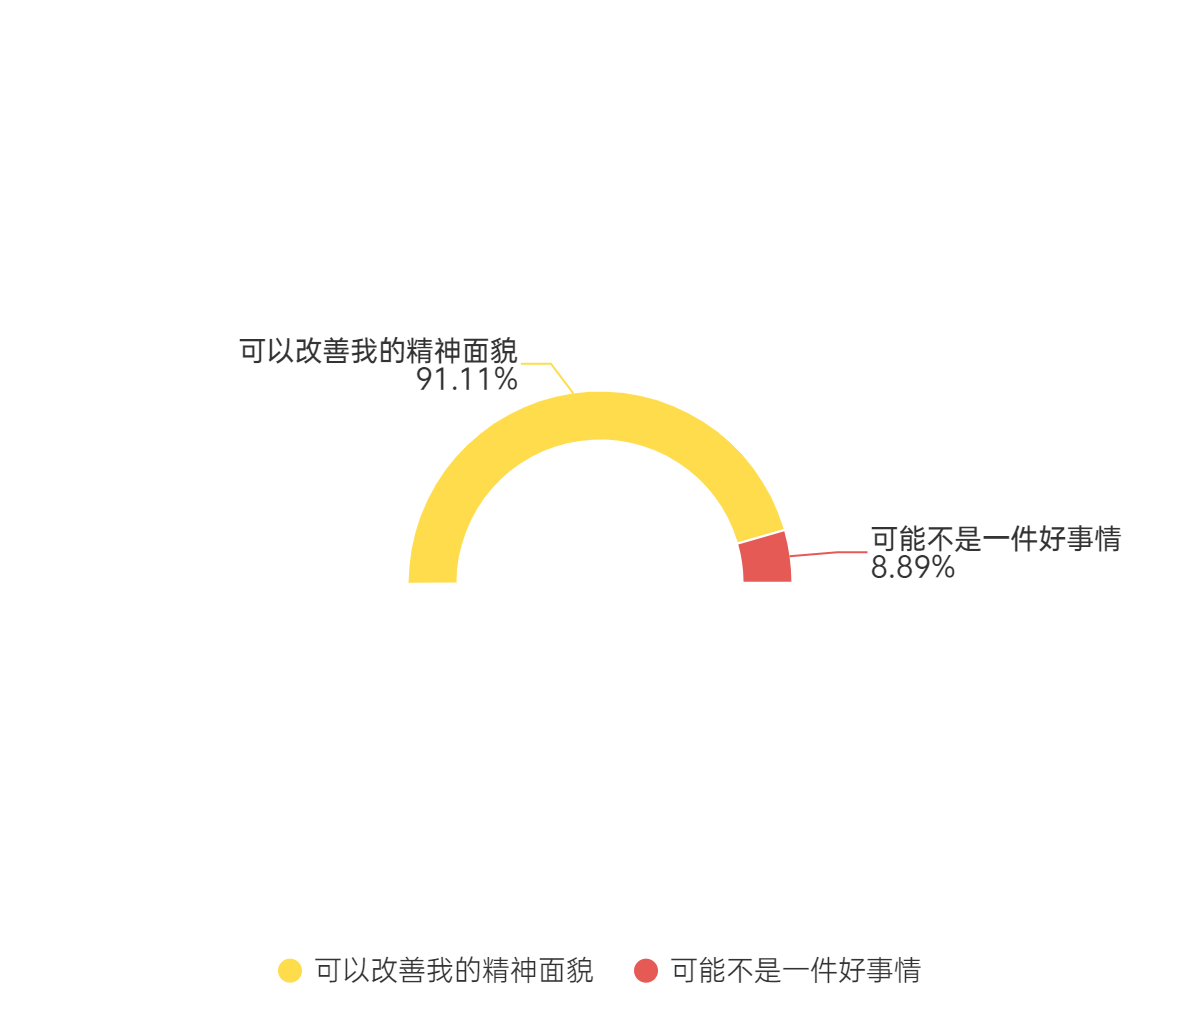
\includegraphics[width=.4\textwidth]{./pic/整理容貌的看法.png}
    \caption{整理容貌的看法}
\end{figure}
\subsection{对容貌焦虑的解决办法及效果}
仅少数同学选择暂时忽略问题,大部分同学选择主动解决,他们表现出积极向好的心态。

大多数表现出容貌焦虑的群体尝试的方法是将关注点转向内在品质,其它解决方法也都取得了不错的效果。
\begin{figure}[H]
    \centering
    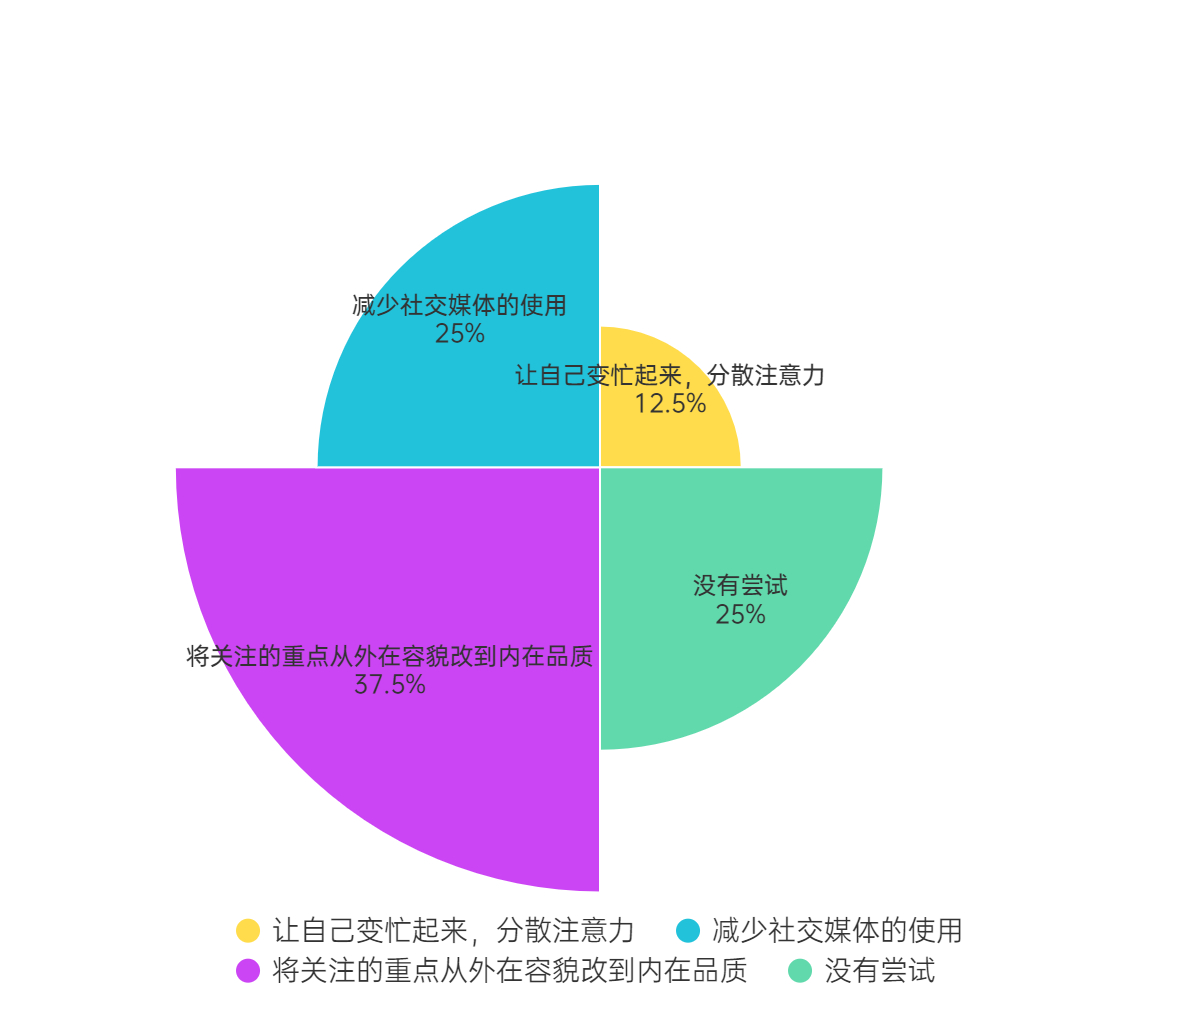
\includegraphics[width=.5\textwidth]{./pic/解决.jpg}
    \caption{对容貌焦虑的解决办法及效果}
\end{figure}
\subsection{总结}
\begin{enumerate}[leftmargin=7em]
    \item 容貌焦虑''现象发生率的性别差异化表现仍然存在,但差异程度有一定的降低。究其原因,可能是因为调查样本主要集中在受教育水平较高且已初步形成较为成熟的价值观的大一学生群体,在自我价值评判体系中,他们会更为重视学识、能力、道德等,也能做到减少外部因素对自身价值观的扭曲。
    \item 大学生群体容貌焦虑的原因主要集中在社会竞争压力上,表明他们可能把面试、面见重要客户这类需要重视容貌的特殊场景过度生活化,同时也有过度抬高容貌在价值体系中的比重的可能,再深入切入也表明大一学生对社会工作认知的切实性不高,其中也可能受到部分影视作品中的戏剧化处理部分的影响,对自我社会竞争力有一定程度上的错误认知。
    \item 大学生群体容貌焦虑的原因还包括美颜技术、医美和化妆品广告及网红宣传以及恋爱的需求,这反映出:部分商家、网红为了利益为``畸形审美''造势,对大学生群体造成了消极影响;部分夸张、悬浮的偶像爱情剧对大学生群体恋爱观的消极影响;大学生容貌焦虑群体在恋爱中一些不愉快体验对他们的恋爱观造成了深刻影响。
    \item 样本中有容貌焦虑表现的大学生群体在日常整理修饰容貌中所花时间并不多,也未表现出明显的想进行医美、化妆的意愿,这也体现出他们的容貌焦虑程度并不高,只是当前一段时间的消极情绪。
    \item 从大一学生群体总体来看,审美健康化已成为主流,他们对容貌的价值认知较为客观理性,遇到问题也多持有积极解决问题的良好心态。
\end{enumerate}
